\part{Theoretische Grundlagen}
\label{sec:theory}

\subsection{Usability}
Web-Performance hat einen großen Einfluss auf die Bedienbarkeit von Webseiten. Ohne die Innovationen im Gebiet der Web-Performance hätte Google mit GMail und ihren anderen Web-Applikationen keinen Erfolg erzielen können. Die Nutzer waren Desktop-Applikationen gew\"ohnt. Nur wenn eine Anwendung auch in einer akzeptablen Geschwindigkeit auf Benutzerinteraktionen reagieren kann, hat sie eine Chance auf dem Markt zu bestehen. Es gibt einige Studien, die sich mit Web-Usability auseinandersetzen. Zu den Ergebnissen gehörte unter anderem, dass langsamere Webseiten zu Vertrauensverlust sowie Nutzerfrustration führen. Als weitere Konsequenz ist der empfundene Qualitätsverlust zu nennen. Die genannten Punkte führen letztendlich zu niedrigeren Konversionsraten, das heißt, dass weniger Besucher zu Kunden werden. Zus\"atzlich steigt die Bail-out-Rate, welche beschreibt, wie viele Nutzer die Webseite w\"ahrend des Ladevorganges wieder verlasssen. 
%http://searchenginewatch.com/article/2085970/Why-Marketers-Must-Care-About-Site-Speed

\subsection{Google Ranking}
Für (Internet-)Firmen ist es von immenser Bedeutung gefunden zu werden. Ein Großteil der Internetnutzer sucht Angebote über die Google-Suche.
%http://www.hitwise.com/us/datacenter/main/dashboard-23984.html
Google hat mit ihrer Initiative "`Let's make the web faster"'\footnote{\url{http://code.google.com/intl/de/speed/}} für viel Entwicklung und Aktivität im Bereich Web-Performance gesorgt und arbeitet zielgerichtet weiter in diese Richtung. Dazu gehören seit 2008 Google AdWords und seit 2010 die Google Suche selbst. Dies stellt viele Unternehmen vor die Aufgabe, ihre Webseite zu optimieren und zu beschleunigen, um im Google-Ranking konkurrenzfähig zu bleiben. Wie genau Google die Webseiten testet, ist nur zum Teil bekannt, da diese Informationen zu Googles Geschäftsgeheimnissen gehören. Es finden sich aber einige Fakten, die bei der Optimierung für die Google-Suche, im Bereich Web-Performance, helfen können.
Bekannt ist, dass der Google-Suchmaschinen-Bot nichts mit der Geschwindigkeitsmessung zu tun hat und Google nur Daten von echten Nutzern, die die Google-Toolbar in ihrem Browser installiert haben, nutzt. Leider sind Daten nur für Internet Explorer ab Version 6 und Firefox ab Version 2 verfügbar. Als Kriterium für die Bewertung wird die Onload-Zeit gemessen. Dabei führt das verzögerte Nachladen von Inhalten zu einem besseren Ergebnis. Wenn eine Webseite für Google optimiert werden soll, muss also auch die Performance mit berücksichtigt werden. Performance ist aber nur ein Teil des Google-Rankings. Für Webseitenbetreiber gilt daher, dass aktuelle und gut strukturierte Inhalte nicht hinter die Performance gestellt werden dürfen.
%http://www.webperformancetoday.com/2011/08/05/faqs-google-seo-search-ranking-website-speed/

\subsection{Serverlast}
Eine umfassende Verbesserung der Auslieferungszeiten von Webseiten hat direkten Einfluss auf die Serverperformance. Dies ist leicht in einem Experiment feststellbar, wie folgende Überlegung zeigt: Wenn eine Webseite nur noch die Hälfte der Zeit benötigt, um ausgeliefert zu werden, hat man doppelt soviel Auslieferungskapazität zur Verfügung. Das spart Kosten für Server und Traffic. Außerdem ermöglichen Caching und Optimierungen einen Großteil an Prozessorlast einzusparen, der dann für andere Aufgaben zur Verfügung steht. Besonders wichtig ist die Performance in Momenten hoher Zugriffszahlen, beispielsweise wenn eine Webseite in einem prominenten News-Portal erwähnt wird. Oftmals bricht dann die Webseite zusammen, weil die Administratoren nicht mit solch einem Ansturm gerechnet haben. Erwähnenswert ist das Newsportal www.heise.de auf dem regelmäßig davon gesprochen wird, es wurde eine Webseite "`geheist"'\footnote{Eine Webseite wurde durch die hohe Anzahl der Zugriffe von Heise-Lesern \"uberlastet.}. Noch problematischer wird es, wenn ein Unternehmen Ziel krimineller Aktivitäten wird. Aktuell zu beobachten ist dieses Phänomen bei den Angriffen des Miner-Botnetzes\footnote{\url{http://www.kaspersky.com/de/news?id=207566473}} auf mehrere deutsche Webseiten. Um sich vor solchen Distributed Denial of Service Angriffen schützen zu können, ist eine performante Webseite sehr wichtig, um genug Ressourcen für Firewalls und andere Gegenmaßnahmen zur Verfügung zu haben.

%\section{Performance Bottlenecks}
\section{Einordnung von Performanzproblemen}
Als Entwickler beziehungsweise Betreiber einer Web-Applikation k\"onnen vielf\"altige Problematiken auftreten. Diese kann man in clientseitige sowie serverseitige Probleme unterteilen. Oft lassen sich diese mit Investitionen in die Infrastruktur beheben. Meistens gibt es aber auch Ans\"atze die durch effizientere Techniken f\"ur Verbesserung sorgen. Dieser Abschnitt versucht die Problemstellungen und Ans\"atze f\"ur Verbesserungen aufzuzeigen.
\subsection{Clientseitige Probleme}
Auf der Client-Seite hat der Applikations-Anbieter die wenigste Kontrolle. Dadurch dass die Applikation im Web angeboten wird m\"ussen die Begleitumst\"ande ber\"ucksichtig werden und es muss klar sein f\"ur welche Frontends programmiert und optimiert werden muss.  
\subsubsection{Netzwerkverbindung}
Die Netzwerkverbindung, als Verbindungsglied zwischen Client und Server, kann an mehreren Stellen f\"ur Probleme sorgen. Betrachtet werden m\"ussen Bandbreite und Latenzen. Latenzen entstehen durch die Wege, die die Informationen zur\"ucklegen m\"ussen und durch Verarbeitung in den Netzwerkknoten. Dass bedeutet besonders f\"ur international ausgerichtete Webseiten, je weiter der Webseitenbesucher physisch entfernt ist, desto langsamer wird die Webseite geladen. Bandbreitenprobleme werden gerade in Deutschland noch durch den mangelhaften Breitbandausbau beg\"unstigt. Daher m\"ussen Webseitenbetreibern auf die Größe der Webseite, die sie an ihre Betrachter ausliefern, Wert legen. Auf folgender Karte wird deutlich, wie sp\"arlich beispielsweise die neuen Bundesl\"ander mit 16 Mbit/s oder mehr versorgt werden. Nur in den dunkelgrün markierten Gebieten werden die Haushalte zuverlässig mit schnellem Internet versorgt.
\begin{figure}[htbp]
  \centering
  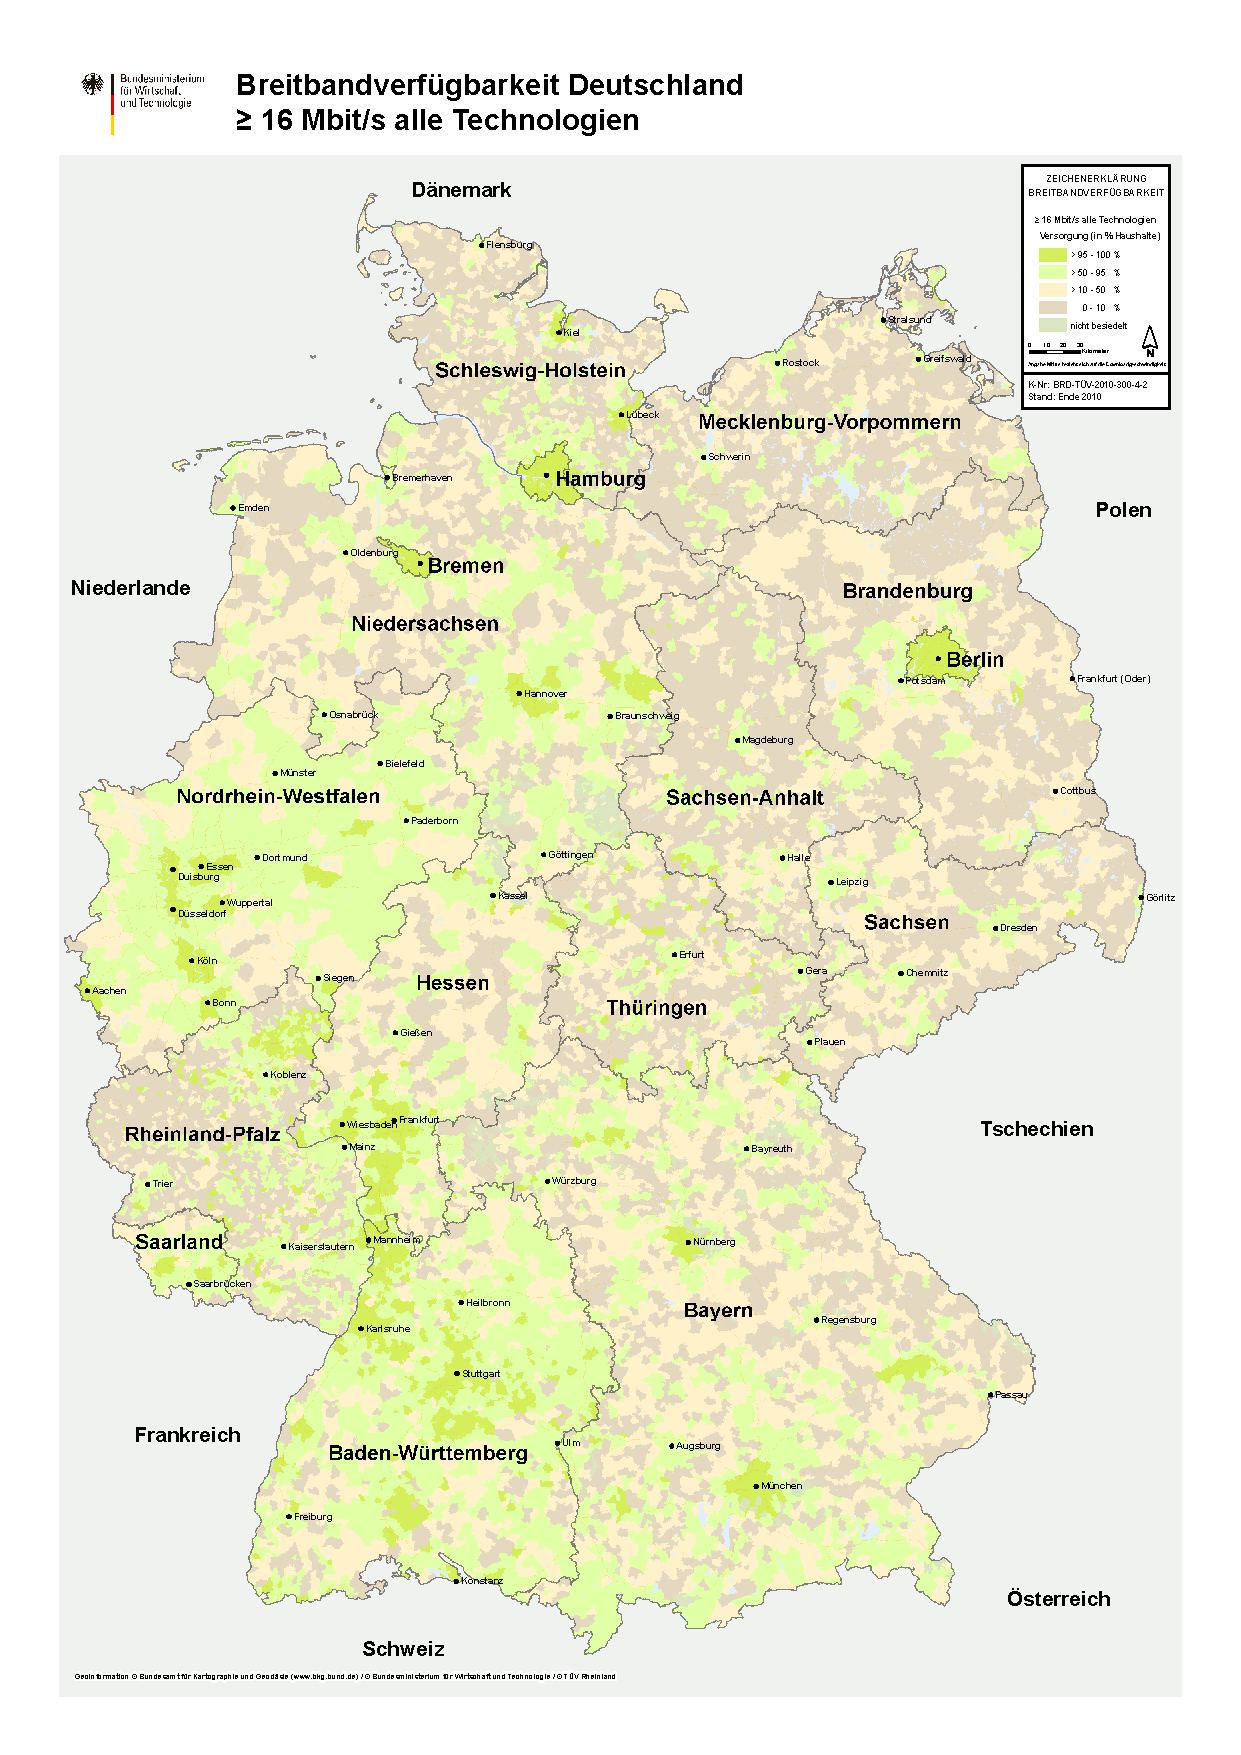
\includegraphics[scale=0.5]{material/breitband201116mbit.pdf}
  \caption{Breitbandversorgung mit 16Mbit/s oder mehr}
  \label{fig:breitband}
\end{figure}
%http://gizmodo.com/5390014/internet-speeds-and-costs-around-the-world-shown-visually
In der Infografik, die aus dem Internet World Stats Broadbrand Penetration Report der IWTF von 2009 abgeleitet wurde, sieht man Deutschland im Vergleich zu den führenden Industrienationen. Der Unterschied zu unserem Nachbarland Frankreich ist sehr deutlich zu erkennen. Auf dem 14. Platz mit ca 5Mbit/s gibt es noch viel Aufholbedarf.
\begin{figure}[htbp]
  \centering
  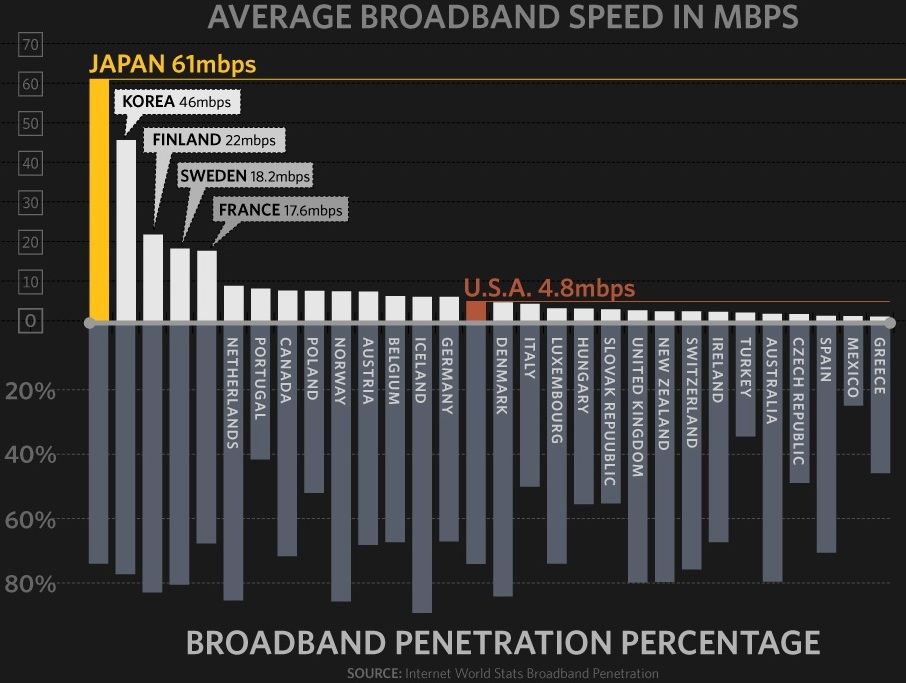
\includegraphics[scale=0.5]{material/worldinternetcomp.jpg}
  \caption{Ausschnitt aus einer Infografik des Internet World Stats Broadbrand Penetration Report der IWTF von 2009 }
  \label{fig:iwtfinfo}
\end{figure}
Um zu verdeutlichen, wie entscheidend die Geschwindigkeit des Internetzugangs für die Ladezeiten einer Webseite ist, folgt ein erläuterndes Beispiel:
Die durchschnittliche Webseitengröße beträgt 320 kB, wie im Abschnitt Ausgangszustand im praktischen Teil erläutert wird. Die üblichsten Anschlussgeschwindigkeiten betragen 1Mbit/s, 2Mbit/s, 6Mbit/s, 16Mbit/s, 25Mbit/s und 50Mbit/s. In der Tabelle wird die Zeit verglichen, die für die Übertragung von 320 kB mit den jeweiligen Bandbreiten, benötigt wird.
\begin{center}
    \begin{longtable}{ l | l | l | l | l | l | l}
    \hline
    Mbit/s & 1 & 2 & 6 & 16 & 25 & 50 \\ \hline
    \hline
	s für 320 kB & 2,6 & 1,3 & 0,44 & 0,16 & 0,1 & 0,05 \\ \hline
    \end{longtable}
\end{center}
Wenn die Ergebnisse in Relation zu den üblichen Ladezeiten im einstelligen Sekundenbereich gebracht werden, wird deutlich, wie groß der Einfluss der Bandbreite im ungünstigsten Fall werden kann.
\subsubsection{Browser}
Als Schnittstelle zwischen Nutzer und Webseite ist der Browser ein besonders kritischer Punkt und muss bei Web-Performanceanalysen besonders beachtet werden.Die meistgenutzten Browser sind der Internet Explorer, Mozilla Firefox, Google Chrome, Opera und Safari. In der folgenden Statistik wird deutlich, dass der Internet Explorer, trotz der oft schlechteren Leistung, Marktführer ist.
\begin{figure}[htbp]
  \centering
  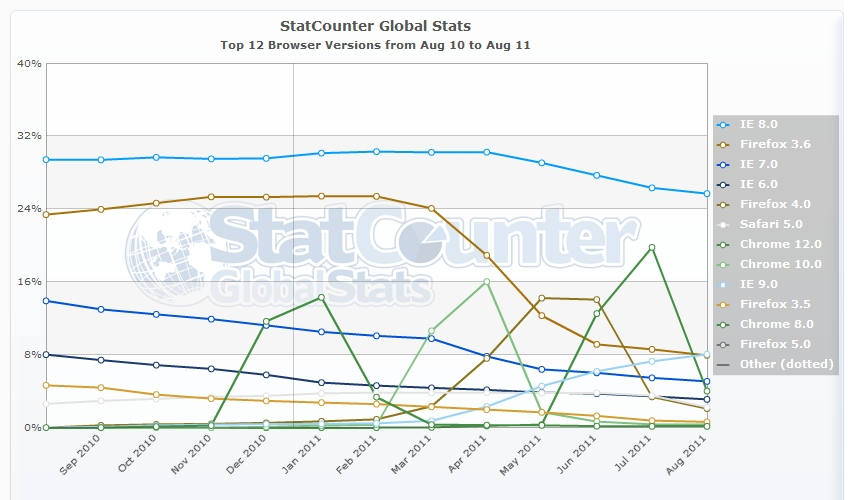
\includegraphics[scale=0.5]{material/browseranteil.jpg}
  \caption{Marktanteile der Browser von August 2010 bis August 2011 http://gs.statcounter.com/#browser_version-ww-monthly-201008-201108}
  \label{fig:browseranteil}
\end{figure}
Für Entwickler bedeutet die Browser-Vielfalt zusätzlichen Entwicklungsaufwand. Unrühmlichstes Beispiel ist der Internet Explorer 6.\footnote{Auszug aus Bugs des Internet Explorer 6:\url{http://www.dosonaro.com/6-der-haeufigsten-ie-bugs-und-wie-man-sie-behebt/}} Seine Kompatibilitätsprobleme sind so schwerwiegend, dass mittlerweile auch vom Hersteller Microsoft ein Update drigendst empfohlen wird.\footnote{Internet Explorer 6 Countdown: \url{http://www.ie6countdown.com/}} Um die Standardkompatibilität zu messen wurden die Acid\footnote{\url{http://www.acidtests.org/}} Tests entwickelt. Der Internet Explorer 6 schafft im Acid3\footnote{Acid3 Test:\url{http://acid3.acidtests.org/}}-Test nur 11/100 Punkten. Moderne Browser wie Google Chrome und auch der Internet Explorer 9 schaffen Werte über 90/100 Punkten. Neben Kompatibilität haben noch andere Leistungsparameter Einfluss auf die Ladezeiten. Die Javascript Ausführungszeiten kann man unter anderem mit dem SunSpider JavaScript Benchmark\footnote{\url{http://www.webkit.org/perf/sunspider/sunspider.html}} testen. Ein Vergleich aktueller Browser zeigt, dass die Browserhersteller versuchen ein einheitlich gutes Level zu erreichen.  
\begin{figure}[htbp]
  \centering
  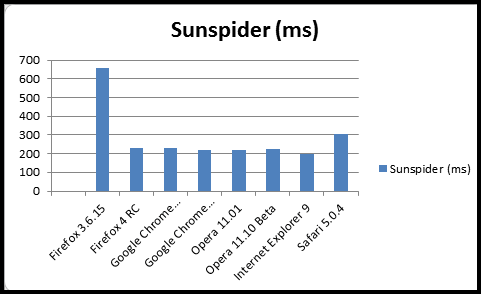
\includegraphics[scale=0.5]{material/sunspiderbenchmark.jpg}
  \caption{SunSpider Benchmark der letzten Browsergeneration}
  \label{fig:sunspider}
\end{figure}
Ein weiterer limitierender Faktor ist die künstliche Beschränkung der parallelen HTTP Zugriffe durch den HTTP/1.1 Standard. In diesem Standard wird festgehalten, dass ein Client die Anzahl paralleler Verbindungen auf 2 beschränken soll. %http://www.ietf.org/rfc/rfc2616.txt 8.1.4
Das bedeutet das mehr Overhead zwischen den Übertragungen entsteht, und der Inhalt nicht komplett parallel heruntergeladen werden kann. Diese Beschränkungen sind eingeführt wurden, da die Prozessorlast mit der Anzahl der Verbindungen zunimmt. Außerdem benötigen die Server mehr Arbeitsspeicher wenn sie zusätzliche Verbindungen aufbauen sollen. Da sich mit der Zeit die Einstellung zu diesem Thema geändert hat ermöglichen aktuelle Browser sechs bis acht parallele Verbindungen, um die Bandbreite der Nutzer auslasten zu können. DOM-Elemente sind 
\begin{itemize}
  \item Anzahl von zu berechnenden DOM-Elementen %TODO was ist DOM
  \item Javascript Ausführungszeiten
  \item Anzahl benötigter HTTP Zugriffe %z.B. Stylesheets Bilder  Warum ist das ein Problem
\end{itemize}

\subsubsection{DOM Elemente}
\subsection{Serverseitig}
% moderne dynamische Webanwendungen sind komplexe Applikationen


\subsubsection{Datenbankabfragen}
So gut wie jede Website nutzt mittlerweile Datenbanken zur Verwaltung ihrer Datenbeständen.

Oft sind diese Datenbanken ein Schwachpunkt für die Web-Performance, da meistens Daten von der Festplatte gelesen werden müssen und komplexe Abfragen viel Zeit in Anspruch nehmen können.

% (Tablelocking Nutzer gleichzeitig)
\subsubsection{Skriptausführung}
\subsubsection{Skriptkompilierung}

\section{Technologiestack und Optimierungsmöglichkeiten}
Im Rahmen dieser Bachelorarbeit werden verschiedenste Technologien verwendet und auf ihnen aufbauende Werkzeuge zu Hilfe genommen. Um zu verstehen wo Probleme lokalisiert sind und wie solche Schwachstellen zu finden sind muss man sich mit dem vorhandenem Technologiestack auseinandersetzen und ihn analysieren.
\begin{description}
  \item[Server] Ein Server ist ein Computer, der Informationen und Dienste für andere Computer zur Verfügung stellt
  \item[Betriebssystem] Die Software die auf dem Server läuft. In der pludoni GmbH wird das Linuxderivat Debian eingesetzt.
  \item[Datenbank] Als Datenbank wird eine strukturierte Sammlung von Daten bezeichnet. Einer der häufigsten Vertreter, gerade im Zusammenhang mit PHP-Webanwendungen, ist MySQL
  \item[Web Server] Der Web Server ist für die zuverlässige Auslieferung von Webseiten zuständig. Er beantwortet die Anfragen die die Nutzer mit dem Browser stellen. Apache2 wird dafür in der pludoni GmbH eingesetzt.
  \item[PHP] ist eine dynamische typisierte Programmiersprache, zur Erstellung von Webanwendungen. %TODO Features von PHP, 
  \item[Drupal] Drupal ist ein CMS und Framework, welches in PHP geschrieben ist und viele direkt nutzbare Funktionen mitbringt. Dazu gehören unter anderem Administrationsoberflächen, Newsaggregatoren, Veröffentlichungsabläufe für Artikel und Blogbeiträge sowie Suchmaschinenoptimierungen. Außerdem ermöglicht Drupal die Installation weiterer, durch Nutzer entwickelte, Module. Dadurch wird eine fast unbegrenzte Funktionsvielfalt ermöglicht. Im vorliegenden Fall wird Drupal in der Version 5 eingesetzt.
  \item[Client] Im Browser der Nutzer kommt am Ende HTML an, dies wird durch Drupal generiert und vom Webserver ausgeliefert. Dabei werden Bilder verarbeitet Javascript Programme ausgeführt und andere Elemente wie Flashapplikationen und Videos berechnet. 
\end{description}

%TODO Bildchen vom Ablauf!

\subsection{Server}
\subsection{PHP}
\subsection{Drupal (5)}
Drupal ist ein Content-Management-System, dass heißt es ermöglicht dem Nutzer eine dynamische Webseite zu erstellen ohne spezielle Programmierkenntnisse zu besitzen. 

% Ist sowohl CMS als auch Framework
\subsection{Benchmark - Werkzeuge}
\subsection{Debugger / Profiler}
\section{Methoden der Web-Performance Optimierung}
Die Methoden zur Leistungssteigerung können wie im Technologiestack untergliedert werden und jedes Element muss für sich betrachtet werden.

\begin{description}
  \item[Serverhardware] Der einzige Parameter der am Server verbessert werden kann ist seine Leistung, dass heißt Datendurchsatz und Rechengeschwindigkeit. Dies geschieht durch CPU Upgrades oder Arbeitsspeichererweiterung. Weitergehend kann man die Festplattenzugriffsgeschwindigkeiten durch RAID Verbünde und neue Technologien wie SSD Speicher verbessern. 
  % Replikation also mehrere Server Load Balancer
  \item[Betriebssystem] Ansatzpunkte für Verbesserungen auf Betriebssystemebene sind Memory-Mapping, dass heißt Speicherbereiche die normalerweise auf der Festplatte liegen werden in den Arbeitsspeicher umgelagert um die Latenzen zu verringern. Dies wird genutzt um Caches zu beschleunigen, die normalerweise von der Festplatte lesen.
  \item[Datenbank] Auf Datenbankebene kann im Fall von MySQL nur beschränkt optimiert werden. Zum einen sind Indizes anzulegen bei häufig genutzten Tabellen und zum anderen kann man MyISAM statt InnoDB nutzen um performanter zu sein.
  % Replikation also mehrere DB Server
  \item[Web Server] Optimierungen am Webserver sind sehr schwierig da die Webserver Performance hauptsächlich von der Serverleistung abhängt. Die Anzahl der gleichzeitigen Zugriffe wird maßgeblich durch den verfügbaren Arbeitsspeicher und die verfügbare Bandbreite eingeschränkt.
  \item[PHP] 
    % Neukomilierung verhindern
    % Clevere Programmierung, Wahl der Frameworks
  \item[Drupal] 
    % Caching 
    % Anzahl der Module, 
    % CSS Aggregation
  \item[HTML] 
    % Caching 
\end{description}